% !BIB TS-program = biber
%%%%%%%%%%%%%%%%%%%%%%%%%%%%%%%%%%%%%%%%%%%%%%%%%%%%%%%%%%%%%%%%%%%%%%%%%%%%%%%%%%%%%%%%%%%%%%%%%%%%%%%%%%%%%%%%%%%%%%%%%%%%%%%%%%%%%%%%%%%%%%%%%%%%%%%%%%%
% This is just an example/guide for you to refer to when producing your supplementary material for your Frontiers article.                                 %
%%%%%%%%%%%%%%%%%%%%%%%%%%%%%%%%%%%%%%%%%%%%%%%%%%%%%%%%%%%%%%%%%%%%%%%%%%%%%%%%%%%%%%%%%%%%%%%%%%%%%%%%%%%%%%%%%%%%%%%%%%%%%%%%%%%%%%%%%%%%%%%%%%%%%%%%%%%

%%% Version 2.5 Generated 2018/06/15 %%%
%%% You will need to have the following packages installed: datetime, fmtcount, etoolbox, fcprefix, which are normally inlcuded in WinEdt. %%%
%%% In http://www.ctan.org/ you can find the packages and how to install them, if necessary. %%%
%%%  NB logo1.jpg is required in the path in order to correctly compile front page header %%%

\documentclass[utf8]{frontiers_suppmat} % for all articles
\usepackage{url,hyperref,lineno,microtype}
\usepackage[onehalfspacing]{setspace}

% bibliography
\usepackage[english]{babel}
\usepackage{csquotes}
\usepackage[
backend=biber, 
bibencoding=utf8, 
style=authoryear, 
date=year, 
maxbibnames=6, 
minbibnames=6, 
url=false, 
isbn=false, 
eprint=false,
uniquename = false, 
autocite=inline]{biblatex}
\addbibresource{conductances.bib}

% make pretty MATLAB code
\usepackage{listings}
\usepackage{matlab-prettifier}
\lstMakeShortInline[style=Matlab-editor]"



% Leave a blank line between paragraphs instead of using \\

\begin{document}
\onecolumn
\firstpage{1}

\title[Supplementary Material]{{\helveticaitalic{Supplementary Material}}:
\\ \helvetica{xolotl: An Intuitive and Approachable Neuron \& Network Simulator in MATLAB}} %Please insert the title of your article here


\maketitle


\section{Database of Conductances}

	Dynamics for model conductances in the following papers have been implemented in "xolotl".
	
	\begin{enumerate}
		\item EAGes, EAGmut, EAGwt (\cite{bronkRegulationEagCa22018})
		\item A-type (\cite{brookingsAutomaticParameterEstimation2014})
		\item Proctolin modulatory input current (\cite{caplanManyParameterSets2014})
		\item CaT, H, Kd, NaV (\cite{dethierPositiveFeedbackCellular2015})
		\item CaL, CaPump, KCa, Kd, NaV (\cite{drionDopaminePacemakerNeuron2017})
		\item Ap, At, Cal, KCa, KCaT, Proc (\cite{goldmanGlobalStructureRobustness2001})
		\item Shaker (\cite{hardieNovelPotassiumChannels1991})
		\item A novel potassium conductance, Shab, Shaker (\cite{herasModulationVoltagedependentConductances2018})
		\item A-type, CaS, CaT, H, KCa, Kd, NaV (\cite{kisperskyIncreaseSodiumConductance2012})
		\item NaP, NaT (\cite{linActivityDependentAlternativeSplicing2012})
		\item A-type, CaS, CaT, H, KCa, Kd, NaV (\cite{liuModelNeuronActivityDependent1998})
		\item \cite{liuModelNeuronActivityDependent1998} conductances with cached gating functions
		\item \cite{liuModelNeuronActivityDependent1998} conductances with forward Euler integration
		\item \cite{liuModelNeuronActivityDependent1998} conductances with temperature dependence (\textit{cf.} \cite{caplanManyParameterSets2014})
		\item Kd and NaV conductances from Int1, LG, and MCN1 cells (\cite{nadimFrequencyRegulationSlow1998})
		\item Calcium current (\cite{nadimSynapticDepressionCreates1999})
		\item Drosophila NaV (\cite{odowdVoltageclampAnalysisSodium1988})
		\item A-type, CaS, CaT, H, KCa, Kd, NaV (\cite{prinzAlternativeHandtuningConductancebased2003})
		\item \cite{prinzAlternativeHandtuningConductancebased2003} conductances with cached gating functions
		\item \cite{prinzAlternativeHandtuningConductancebased2003} conductances with temperature dependence (\textit{cf.} \cite{caplanManyParameterSets2014})
		\item Kd and NaV from Int1 cells and modulatory input and transient LTS conductances from LG cells (\cite{rodriguezConvergentRhythmGeneration2013})
		\item Proctolin modulatory input (\cite{sharpDynamicClampComputergenerated1993})
		\item Cal and Kd from AB-PD, LP, and PY cells (\cite{soto-trevinoActivitydependentModificationInhibitory2001})
		\item A-type, CaT, and KCa from AB and PD cells, generic H, Kd, NaP, NaV, and proctolin conductances (\cite{soto-trevinoComputationalModelElectrically2005})
		\item Proctolin modulatory input (\cite{swensenModulatorsConvergentCellular2001})
		\item A-type, CaS, CaT, H, KCa, Kd, NaP, NaV (\cite{turrigianoSelectiveRegulationCurrent1995})
		\item Drosophila NaV (\cite{wicherNonsynapticIonChannels2001})
	\end{enumerate}

\section{Parameters for Simulations}

	Two single-compartment models were simulated in this paper. The first, a Hodgkin-Huxley model with three conductances ("NaV", "Kd", and "Leak") and injected current was simulated for Figure 1 and 7. The second is a stomatogastric neuron model with eight conductances ("NaV", "CaT", "CaS", "ACurrent", "KCa", "Kd", "HCurrent", "Leak") and was simulated for Figure 3 and 7. Both models have dynamics as described in \cite{liuModelNeuronActivityDependent1998}.
	
	\subsection{Parameters for Hodgkin-Huxley model} 
	
		\begin{center}
			\begin{tabular}{|l|r|l|}
				\hline 
				\textbf{Parameter Name} & \textbf{Value} & \textbf{Units} \\ 
				\hline 
				Membrane capacitance ("HH.Cm") & 10 & ${nF}/{mm^2}$ \\ 
				\hline 
				Surface area ("HH.A") & 0.01 & $mm^2$ \\ 
				\hline 
				Fast sodium maximal conductance ("HH.NaV.gbar") & 1000 & $\mu S/mm^2$ \\ 
				\hline 
				Delayed rectifier maximal conductance ("HH.Kd.gbar") & 300 & $\mu S/mm^2$ \\ 
				\hline 
				Passive leak maximal conductance ("HH.Leak.gbar") & 1 & $\mu S/mm^2$ \\ 
				\hline 
				Sodium reversal potential ("HH.NaV.E") & 50 & $mV$ \\ 
				\hline 
				Potassium reversal potential ("HH.Kd.E") & -80 & $mV$ \\ 
				\hline
				Leak reversal potential ("HH.Leak.E") & -50 & $mV$ \\
				\hline
				Injected current ("I_ext") & 0.2 & $nA$ \\
				\hline 
			\end{tabular} 
		\end{center}
	
	\subsection{Parameters for Stomatogastric Model}
	
		\begin{center}
			\begin{tabular}{|l|r|l|}
				\hline 
				\textbf{Parameter Name} & \textbf{Value} & \textbf{Units} \\ 
				\hline 
				Membrane capacitance ("AB.Cm") & 10 & ${nF}/{mm^2}$ \\ 
				\hline 
				Surface area ("AB.A") & 0.0628 & $mm^2$ \\
				\hline
				Calcium buffering $\phi$ ("AB.phi") & 90 & $\mu M / nA$ \\
				\hline
				Calcium buffering shell volume ("AB.vol") & 0.0628 & $mm^3$ \\
				\hline 
				Fast sodium maximal conductance ("AB.NaV.gbar") & 1831.2 & $\mu S/mm^2$ \\ 
				\hline
				Transient calcium maximal conductance ("AB.CaT.gbar") & 22.93 & $\mu S/mm^2$ \\ 
				\hline 
				Slow calcium maximal conductance ("AB.CaS.gbar") & 27.07 & $\mu S/mm^2$ \\ 
				\hline 
				Transient potassium maximal conductance ("AB.ACurrent.gbar") & 246.02 & $\mu S/mm^2$ \\ 
				\hline 
				Calcium-gated potassium maximal conductance ("AB.KCa.gbar") & 979.94 & $\mu S/mm^2$ \\ 
				\hline 
				Delayed rectifier maximal conductance ("AB.Kd.gbar") & 610.03 & $\mu S/mm^2$ \\ 
				\hline
				Hyperpolarization-activated maximal conductance ("AB.HCurrent.gbar") & 10.1 & $\mu S/mm^2$ \\ 
				\hline 
				Passive leak maximal conductance ("AB.Leak.gbar") & 0.99045 & $\mu S/mm^2$ \\ 
				\hline 
				Sodium reversal potential ("AB.NaV.E") & 30 & $mV$ \\ 
				\hline 
				Potassium reversal potential ("AB.Kd.E") & -80 & $mV$ \\ 
				\hline
				Hyperpolarization-activated reversal potential ("AB.HCurrent.E") & -20 & $mV$ \\
				\hline
				Leak reversal potential ("AB.Leak.E") & -50 & $mV$ \\
				\hline
			\end{tabular} 
		\end{center}

	\subsection{Parameters for Network Model}
		The network model displayed in Figure 4 is described in \cite{prinzAlternativeHandtuningConductancebased2003, prinzSimilarNetworkActivity2004}. It is comprised of three compartments "AB", "LP", and "PY" with the same dynamics but differing parameters and synaptic inputs.
		
		\begin{center}
			\begin{tabular}{|l|c|c|c|c|}
				\hline 
				\textbf{Parameter Name} & \textbf{AB} & \textbf{LP} & \textbf{PY} & \textbf{Units} \\ 
				\hline 
				Fast sodium maximal conductance & 1000 & 1000 & 1000 & $\mu S/mm^2$ \\ 
				\hline 
				Transient calcium maximal conductance & 25 & 0 & 24 & $\mu S/mm^2$ \\  
				\hline 
				Slow calcium maximal conductance & 60 & 40 & 20 & $\mu S/mm^2$ \\  
				\hline 
				Transient calcium maximal conductance & 500 & 200 & 500 & $\mu S/mm^2$ \\  
				\hline 
				Calcium-gated potassium maximal conductance & 50 & 0 & 0 & $\mu S/mm^2$ \\  
				\hline 
				Delayed rectifier maximal conductance & 1000 & 250 & 1250 & $\mu S/mm^2$ \\  
				\hline 
				Hyperpolarization-activated maximal conductance & 0.1 & 0.5 & 0.5 & $\mu S/mm^2$ \\  
				\hline 
				Leak maximal conductance & 0 & 0.3 & 0.1 & $\mu S/mm^2$ \\  
				\hline 
				Sodium reversal potential & 50 & 50 & 50 & $mV$ \\ 
				\hline 
				Potassium reversal potential & -80 & -80 & -80 & $mV$ \\ 
				\hline
				Hyperpolarization-activated reversal potential & -20 & -20 & -20 & $mV$ \\
				\hline
				Leak reversal potential & -50 & -50 & -50 & $mV$ \\
				\hline
			\end{tabular}
		\end{center}
	
		There are seven synapses in the model of two types: glutamatergic ("Glut") and cholinergic ("Chol") with differing dynamics. The synapse produces a current in the postsynaptic compartment based on the membrane potential in the presynaptic compartment. 
		
		\begin{center}
			\begin{tabular}{|c|c|c|r|}
				\hline
				\textbf{Presynaptic} & \textbf{Postsynaptic} & \textbf{Type} & $\bar{g}$ ($\mu S/mm^2$) \\
				\hline
				AB & LP & Chol & 30 \\ \hline
				AB & PY & Chol & 3 \\ \hline
				AB & LP & Glut & 30 \\ \hline
				AB & PY & Glut & 10 \\ \hline
				LP & PY & Glut & 1 \\ \hline
				PY & LP & Glut & 30 \\ \hline
				LP & AB & Glut & 30 \\ \hline
			\end{tabular}
		\end{center}
	
\section{Stability of Exponential Euler Method}

Bursting models from the Prinz stomatogastric ganglion model database (\cite{prinzAlternativeHandtuningConductancebased2003}) were simulated for 15 seconds at varying time resolution in order to characterize the stability of the exponential Euler numerical integration method. The exponential Euler method is generally accurate up to $\approx 0.1$ ms for most models tested. A time step of $\approx 0.05$ ms gives a good compromise between accuracy and speed (\cite{prinzAlternativeHandtuningConductancebased2003, prinzSimilarNetworkActivity2004}).
	
\begin{figure}
\centering
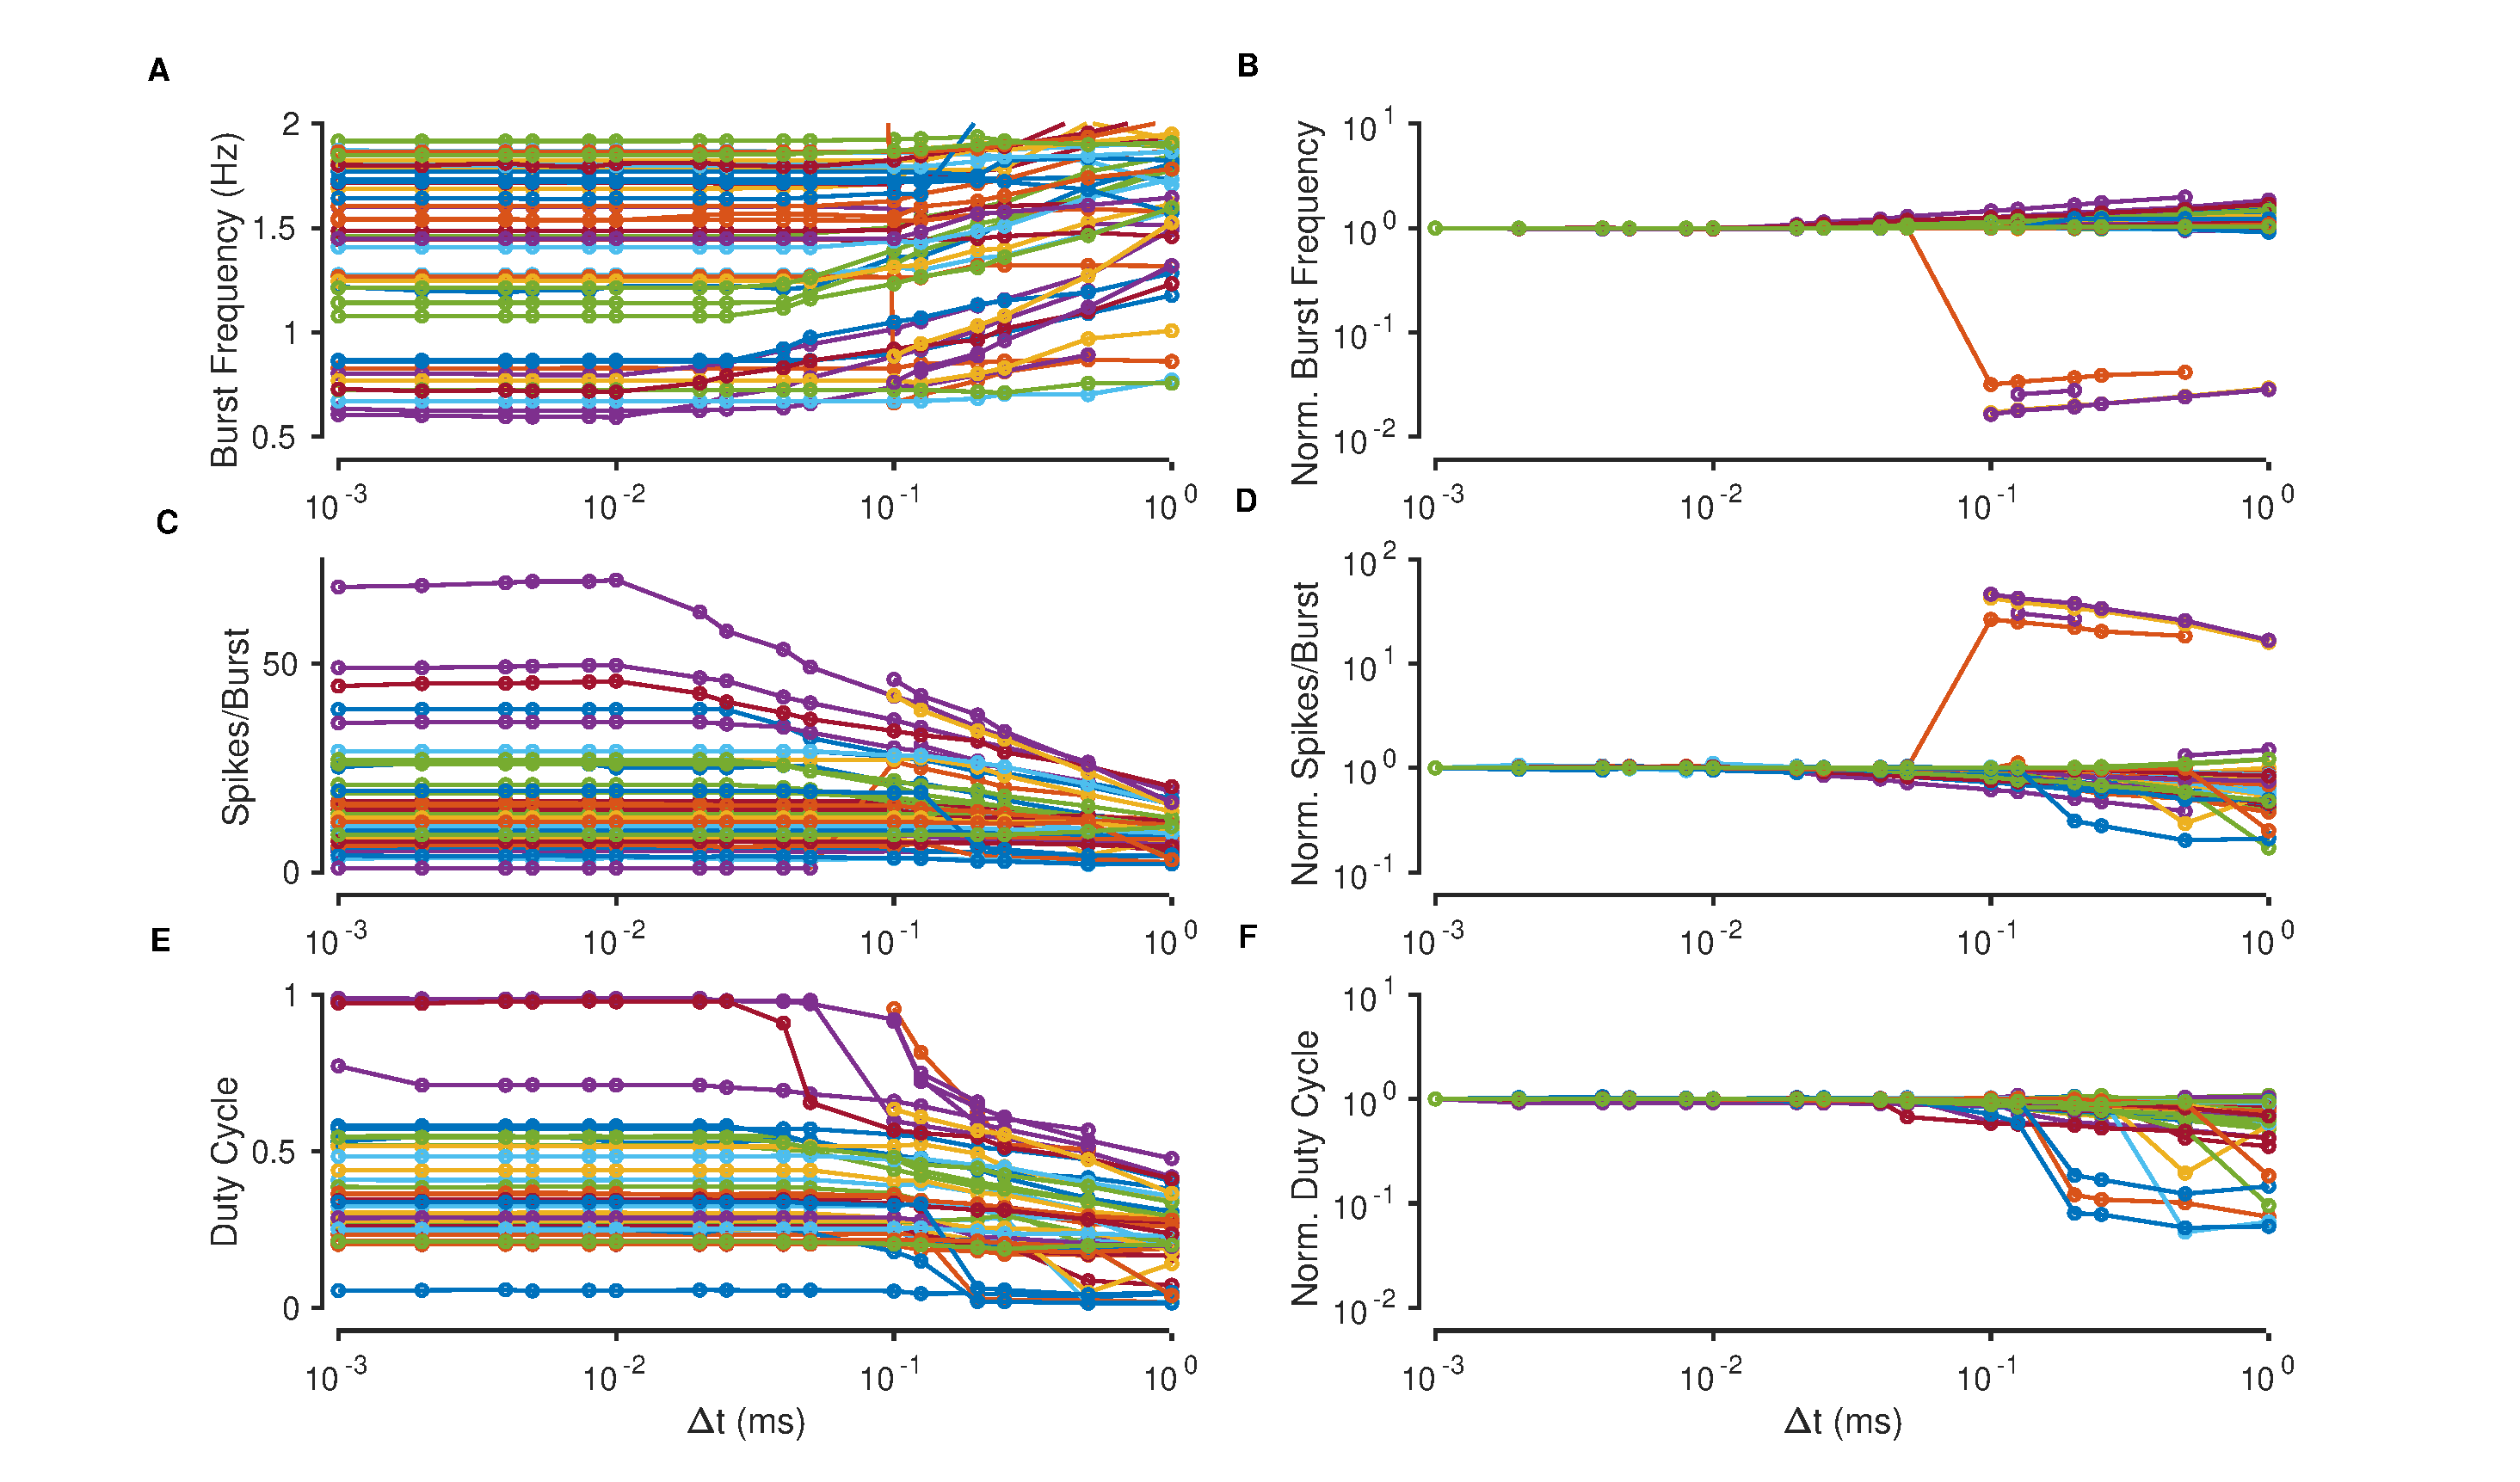
\includegraphics[width=1.0\linewidth]{gfx/figure_sup_stability}
\caption{Stability of exponential Euler method using models randomly chosen from the Prinz database. (A, C, E) Three metrics of bursting neurons: burst frequency, average spikes per burst, and duty cycle were computed over increasing time step. (B, D, F) The metrics were normalized to the first value in for each model. A line of zero slope would indicate no significant change in integration error over increasing time step. Each line indicates a model with different maximal conductances.}
\label{fig:figuresupstability}
\end{figure}

\cleardoublepage

\printbibliography

\end{document}
